% neighbor_diagram_v2.tex -- "Neighborhood" version of the diagram for eq:total-gauss.
% Drawn to scale in um (1 um = 1.25 cm). The gray shading is Omega(d), the weight per unit
% area, linear in gray (omega_rings.tex, written by omega_data.py): it vanishes at r, peaks at
% d = 0.43 um and fades by 1.5 um. Dashed circles: half of the weight lies within 0.68 um, 94%
% within 2 um. Rods (headless) at a few neighbors, each joined to r by a thin gray line (the
% line to r); color by the sign of cos 2(theta_nb - theta_d) as in fig:aimed-rods, opacity
% 0.25 + 0.75 |cos 2(theta_nb - theta_d)|, faint outside 2 um as in fig:aimed-rods.
% Width: natural size, about 171 pt (0.69 of the revtex \linewidth); include it at that size
% (\includegraphics without a width) so the fonts print at 8-9 pt.
% Build with ./run.sh.
\documentclass[tikz,border=0pt]{standalone}
% neighbor_preamble.tex -- shared by neighbor_diagram_v1/v2/v3.tex.
% Notation as in manuscript/definitions.tex: \r = \mathbf{r}, \bs = \boldsymbol,
% \elln = \ell_{\rm n}, \micron = \upmu\mathrm{m}. The body font is Computer Modern, as in
% revtex (no font package), and standalone sets 10 pt, so \small = 9 pt and
% \footnotesize = 8 pt print at those sizes when the pdf is included at its natural width.
\usepackage{amsmath,amssymb,upgreek}
\usepackage{xcolor}
\usepackage{tikz}
\usetikzlibrary{arrows.meta,calc}
\newcommand{\bs}{\boldsymbol}
\renewcommand{\r}{\mathbf{r}}
\newcommand{\elln}{\ell_{\rm n}}
\newcommand{\micron}{\upmu\mathrm{m}}
% the two sign colors of fig:aimed-rods (aimed_rods_exact.wls): the ends of Mathematica's
% TemperatureMap, cmap[0.97] (raises the variance) and cmap[0.03] (lowers it)
\definecolor{plusS}{rgb}{0.832,0.248,0.178}
\definecolor{minusS}{rgb}{0.226,0.355,0.936}
% the curve color of fig:omega-weight (omega_weight.wls)
\definecolor{curve}{rgb}{0.20,0.40,0.70}
\tikzset{
  >={Stealth[length=4.5pt,width=3.6pt]},
  rod/.style={line width=2.2pt, line cap=round},
  ref/.style={gray!75, line width=0.4pt},
  ang/.style={line width=0.5pt},
  pt/.style={fill=white, draw=black, line width=0.8pt},
  dvec/.style={->, line width=0.7pt},
  panel/.style={font=\small\bfseries},
}
% the point r: white disk with a black ring, as in fig:aimed-rods
\newcommand{\pointr}[1]{\filldraw[pt] (#1) circle (2.3pt);}
% the center of a neighbor rod
\newcommand{\nbdot}[1]{\fill (#1) circle (1.3pt);}

% generated by omega_data.py
\def\dmed{0.6822}%  median radius, um
\def\radmed{1.1314}%  2 pi d Omega at the median
\def\dpeak{0.5383}%  peak of 2 pi d Omega, um
\def\radtwo{0.0625}%  2 pi d Omega at 2 um

% \nbrod{phi}{rho}{alpha}: a neighbor at polar angle phi (deg) and distance rho (um) from r,
% its rod at angle alpha = theta_nb - theta_d from the line to r
\newcommand{\nbrod}[3]{%
  \pgfmathsetmacro{\cc}{cos(2*(#3))}%
  \pgfmathsetmacro{\op}{min(1,(#2 > 2 ? 0.30 : 1)*(0.25+0.75*abs(\cc)))}%
  \pgfmathsetmacro{\pos}{\cc > 0 ? 1 : 0}%
  \ifdim\pos pt>0.5pt\def\rodcol{plusS}\else\def\rodcol{minusS}\fi
  \draw[ref, line width=0.35pt, gray!55] (0,0) -- (#1:#2);
  \draw[rod, \rodcol, draw opacity=\op, line width=2.0pt]
    ($(#1:#2)+(#1+#3:\hrod)$) -- ($(#1:#2)-(#1+#3:\hrod)$);
  \fill[draw opacity=\op, opacity=\op] (#1:#2) circle (1.1pt);}
\def\hrod{0.28}
\begin{document}
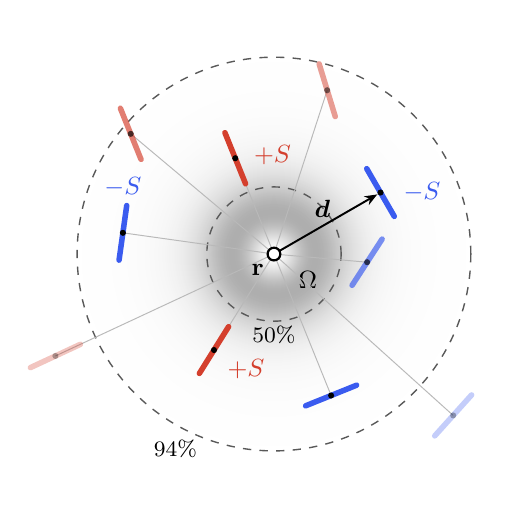
\begin{tikzpicture}[x=1.25cm, y=1.25cm, font=\small]
  % ---------------------------------------------------------------- weight Omega
  % generated by omega_data.py: gray disks, level proportional to Omega(d)
\fill[black!0.00] (0,0) circle (2.300);
\fill[black!0.01] (0,0) circle (2.290);
\fill[black!0.01] (0,0) circle (2.280);
\fill[black!0.01] (0,0) circle (2.270);
\fill[black!0.02] (0,0) circle (2.260);
\fill[black!0.02] (0,0) circle (2.250);
\fill[black!0.03] (0,0) circle (2.240);
\fill[black!0.03] (0,0) circle (2.230);
\fill[black!0.03] (0,0) circle (2.220);
\fill[black!0.04] (0,0) circle (2.210);
\fill[black!0.04] (0,0) circle (2.200);
\fill[black!0.05] (0,0) circle (2.190);
\fill[black!0.05] (0,0) circle (2.180);
\fill[black!0.06] (0,0) circle (2.170);
\fill[black!0.06] (0,0) circle (2.160);
\fill[black!0.07] (0,0) circle (2.150);
\fill[black!0.07] (0,0) circle (2.140);
\fill[black!0.08] (0,0) circle (2.130);
\fill[black!0.08] (0,0) circle (2.120);
\fill[black!0.09] (0,0) circle (2.110);
\fill[black!0.10] (0,0) circle (2.100);
\fill[black!0.10] (0,0) circle (2.090);
\fill[black!0.11] (0,0) circle (2.080);
\fill[black!0.11] (0,0) circle (2.070);
\fill[black!0.12] (0,0) circle (2.060);
\fill[black!0.13] (0,0) circle (2.050);
\fill[black!0.13] (0,0) circle (2.040);
\fill[black!0.14] (0,0) circle (2.030);
\fill[black!0.15] (0,0) circle (2.020);
\fill[black!0.15] (0,0) circle (2.010);
\fill[black!0.16] (0,0) circle (2.000);
\fill[black!0.17] (0,0) circle (1.990);
\fill[black!0.18] (0,0) circle (1.980);
\fill[black!0.18] (0,0) circle (1.970);
\fill[black!0.19] (0,0) circle (1.960);
\fill[black!0.20] (0,0) circle (1.950);
\fill[black!0.21] (0,0) circle (1.940);
\fill[black!0.22] (0,0) circle (1.930);
\fill[black!0.23] (0,0) circle (1.920);
\fill[black!0.24] (0,0) circle (1.910);
\fill[black!0.25] (0,0) circle (1.900);
\fill[black!0.26] (0,0) circle (1.890);
\fill[black!0.27] (0,0) circle (1.880);
\fill[black!0.28] (0,0) circle (1.870);
\fill[black!0.29] (0,0) circle (1.860);
\fill[black!0.30] (0,0) circle (1.850);
\fill[black!0.31] (0,0) circle (1.840);
\fill[black!0.32] (0,0) circle (1.830);
\fill[black!0.33] (0,0) circle (1.820);
\fill[black!0.34] (0,0) circle (1.810);
\fill[black!0.36] (0,0) circle (1.800);
\fill[black!0.37] (0,0) circle (1.790);
\fill[black!0.38] (0,0) circle (1.780);
\fill[black!0.40] (0,0) circle (1.770);
\fill[black!0.41] (0,0) circle (1.760);
\fill[black!0.42] (0,0) circle (1.750);
\fill[black!0.44] (0,0) circle (1.740);
\fill[black!0.45] (0,0) circle (1.730);
\fill[black!0.47] (0,0) circle (1.720);
\fill[black!0.49] (0,0) circle (1.710);
\fill[black!0.50] (0,0) circle (1.700);
\fill[black!0.52] (0,0) circle (1.690);
\fill[black!0.54] (0,0) circle (1.680);
\fill[black!0.56] (0,0) circle (1.670);
\fill[black!0.57] (0,0) circle (1.660);
\fill[black!0.59] (0,0) circle (1.650);
\fill[black!0.61] (0,0) circle (1.640);
\fill[black!0.63] (0,0) circle (1.630);
\fill[black!0.65] (0,0) circle (1.620);
\fill[black!0.68] (0,0) circle (1.610);
\fill[black!0.70] (0,0) circle (1.600);
\fill[black!0.72] (0,0) circle (1.590);
\fill[black!0.75] (0,0) circle (1.580);
\fill[black!0.77] (0,0) circle (1.570);
\fill[black!0.80] (0,0) circle (1.560);
\fill[black!0.82] (0,0) circle (1.550);
\fill[black!0.85] (0,0) circle (1.540);
\fill[black!0.88] (0,0) circle (1.530);
\fill[black!0.91] (0,0) circle (1.520);
\fill[black!0.94] (0,0) circle (1.510);
\fill[black!0.97] (0,0) circle (1.500);
\fill[black!1.00] (0,0) circle (1.490);
\fill[black!1.03] (0,0) circle (1.480);
\fill[black!1.07] (0,0) circle (1.470);
\fill[black!1.10] (0,0) circle (1.460);
\fill[black!1.14] (0,0) circle (1.450);
\fill[black!1.18] (0,0) circle (1.440);
\fill[black!1.22] (0,0) circle (1.430);
\fill[black!1.26] (0,0) circle (1.420);
\fill[black!1.30] (0,0) circle (1.410);
\fill[black!1.34] (0,0) circle (1.400);
\fill[black!1.39] (0,0) circle (1.390);
\fill[black!1.44] (0,0) circle (1.380);
\fill[black!1.48] (0,0) circle (1.370);
\fill[black!1.53] (0,0) circle (1.360);
\fill[black!1.59] (0,0) circle (1.350);
\fill[black!1.64] (0,0) circle (1.340);
\fill[black!1.70] (0,0) circle (1.330);
\fill[black!1.76] (0,0) circle (1.320);
\fill[black!1.82] (0,0) circle (1.310);
\fill[black!1.88] (0,0) circle (1.300);
\fill[black!1.95] (0,0) circle (1.290);
\fill[black!2.02] (0,0) circle (1.280);
\fill[black!2.09] (0,0) circle (1.270);
\fill[black!2.16] (0,0) circle (1.260);
\fill[black!2.24] (0,0) circle (1.250);
\fill[black!2.32] (0,0) circle (1.240);
\fill[black!2.40] (0,0) circle (1.230);
\fill[black!2.49] (0,0) circle (1.220);
\fill[black!2.58] (0,0) circle (1.210);
\fill[black!2.67] (0,0) circle (1.200);
\fill[black!2.77] (0,0) circle (1.190);
\fill[black!2.87] (0,0) circle (1.180);
\fill[black!2.98] (0,0) circle (1.170);
\fill[black!3.09] (0,0) circle (1.160);
\fill[black!3.21] (0,0) circle (1.150);
\fill[black!3.33] (0,0) circle (1.140);
\fill[black!3.45] (0,0) circle (1.130);
\fill[black!3.58] (0,0) circle (1.120);
\fill[black!3.72] (0,0) circle (1.110);
\fill[black!3.87] (0,0) circle (1.100);
\fill[black!4.02] (0,0) circle (1.090);
\fill[black!4.17] (0,0) circle (1.080);
\fill[black!4.34] (0,0) circle (1.070);
\fill[black!4.51] (0,0) circle (1.060);
\fill[black!4.68] (0,0) circle (1.050);
\fill[black!4.87] (0,0) circle (1.040);
\fill[black!5.07] (0,0) circle (1.030);
\fill[black!5.27] (0,0) circle (1.020);
\fill[black!5.48] (0,0) circle (1.010);
\fill[black!5.70] (0,0) circle (1.000);
\fill[black!5.94] (0,0) circle (0.990);
\fill[black!6.18] (0,0) circle (0.980);
\fill[black!6.43] (0,0) circle (0.970);
\fill[black!6.69] (0,0) circle (0.960);
\fill[black!6.97] (0,0) circle (0.950);
\fill[black!7.26] (0,0) circle (0.940);
\fill[black!7.56] (0,0) circle (0.930);
\fill[black!7.87] (0,0) circle (0.920);
\fill[black!8.20] (0,0) circle (0.910);
\fill[black!8.54] (0,0) circle (0.900);
\fill[black!8.89] (0,0) circle (0.890);
\fill[black!9.26] (0,0) circle (0.880);
\fill[black!9.64] (0,0) circle (0.870);
\fill[black!10.04] (0,0) circle (0.860);
\fill[black!10.45] (0,0) circle (0.850);
\fill[black!10.88] (0,0) circle (0.840);
\fill[black!11.32] (0,0) circle (0.830);
\fill[black!11.78] (0,0) circle (0.820);
\fill[black!12.26] (0,0) circle (0.810);
\fill[black!12.75] (0,0) circle (0.800);
\fill[black!13.26] (0,0) circle (0.790);
\fill[black!13.78] (0,0) circle (0.780);
\fill[black!14.32] (0,0) circle (0.770);
\fill[black!14.87] (0,0) circle (0.760);
\fill[black!15.44] (0,0) circle (0.750);
\fill[black!16.02] (0,0) circle (0.740);
\fill[black!16.62] (0,0) circle (0.730);
\fill[black!17.23] (0,0) circle (0.720);
\fill[black!17.85] (0,0) circle (0.710);
\fill[black!18.48] (0,0) circle (0.700);
\fill[black!19.12] (0,0) circle (0.690);
\fill[black!19.77] (0,0) circle (0.680);
\fill[black!20.43] (0,0) circle (0.670);
\fill[black!21.09] (0,0) circle (0.660);
\fill[black!21.75] (0,0) circle (0.650);
\fill[black!22.42] (0,0) circle (0.640);
\fill[black!23.08] (0,0) circle (0.630);
\fill[black!23.74] (0,0) circle (0.620);
\fill[black!24.40] (0,0) circle (0.610);
\fill[black!25.05] (0,0) circle (0.600);
\fill[black!25.69] (0,0) circle (0.590);
\fill[black!26.31] (0,0) circle (0.580);
\fill[black!26.92] (0,0) circle (0.570);
\fill[black!27.50] (0,0) circle (0.560);
\fill[black!28.06] (0,0) circle (0.550);
\fill[black!28.60] (0,0) circle (0.540);
\fill[black!29.11] (0,0) circle (0.530);
\fill[black!29.58] (0,0) circle (0.520);
\fill[black!30.02] (0,0) circle (0.510);
\fill[black!30.41] (0,0) circle (0.500);
\fill[black!30.77] (0,0) circle (0.490);
\fill[black!31.07] (0,0) circle (0.480);
\fill[black!31.33] (0,0) circle (0.470);
\fill[black!31.53] (0,0) circle (0.460);
\fill[black!31.68] (0,0) circle (0.450);
\fill[black!31.76] (0,0) circle (0.440);
\fill[black!31.79] (0,0) circle (0.430);
\fill[black!31.75] (0,0) circle (0.420);
\fill[black!31.65] (0,0) circle (0.410);
\fill[black!31.48] (0,0) circle (0.400);
\fill[black!31.24] (0,0) circle (0.390);
\fill[black!30.92] (0,0) circle (0.380);
\fill[black!30.54] (0,0) circle (0.370);
\fill[black!30.09] (0,0) circle (0.360);
\fill[black!29.57] (0,0) circle (0.350);
\fill[black!28.98] (0,0) circle (0.340);
\fill[black!28.32] (0,0) circle (0.330);
\fill[black!27.59] (0,0) circle (0.320);
\fill[black!26.80] (0,0) circle (0.310);
\fill[black!25.95] (0,0) circle (0.300);
\fill[black!25.04] (0,0) circle (0.290);
\fill[black!24.08] (0,0) circle (0.280);
\fill[black!23.06] (0,0) circle (0.270);
\fill[black!22.00] (0,0) circle (0.260);
\fill[black!20.90] (0,0) circle (0.250);
\fill[black!19.77] (0,0) circle (0.240);
\fill[black!18.60] (0,0) circle (0.230);
\fill[black!17.42] (0,0) circle (0.220);
\fill[black!16.22] (0,0) circle (0.210);
\fill[black!15.01] (0,0) circle (0.200);
\fill[black!13.80] (0,0) circle (0.190);
\fill[black!12.60] (0,0) circle (0.180);
\fill[black!11.41] (0,0) circle (0.170);
\fill[black!10.24] (0,0) circle (0.160);
\fill[black!9.10] (0,0) circle (0.150);
\fill[black!7.99] (0,0) circle (0.140);
\fill[black!6.93] (0,0) circle (0.130);
\fill[black!5.92] (0,0) circle (0.120);
\fill[black!4.97] (0,0) circle (0.110);
\fill[black!4.08] (0,0) circle (0.100);
\fill[black!3.26] (0,0) circle (0.090);
\fill[black!2.52] (0,0) circle (0.080);
\fill[black!1.86] (0,0) circle (0.070);
\fill[black!1.28] (0,0) circle (0.060);
\fill[black!0.79] (0,0) circle (0.050);
\fill[black!0.40] (0,0) circle (0.040);
\fill[black!0.10] (0,0) circle (0.030);
\fill[black!0.00] (0,0) circle (0.020);
\fill[black!0.00] (0,0) circle (0.010);

  \draw[ref, dashed, gray!70!black, line width=0.5pt] (0,0) circle (\dmed);
  \draw[ref, dashed, gray!70!black, line width=0.5pt] (0,0) circle (2);
  \node[font=\footnotesize, anchor=north, inner sep=1.5pt] at (-90:\dmed) {$50\%$};
  \node[font=\footnotesize, anchor=north east, inner sep=1pt] at (-112:2) {$94\%$};
  \node[inner sep=0pt] at (323:0.43) {$\Omega$};
  % ---------------------------------------------------------------- neighbors
  %       phi  rho  alpha
  \nbrod{112}{1.05}{0}
  \nbrod{172}{1.55}{90}
  \nbrod{238}{1.15}{0}
  \nbrod{292}{1.55}{90}
  \nbrod{355}{0.95}{62}
  \nbrod{72}{1.75}{35}
  \nbrod{140}{1.90}{-28}
  \nbrod{205}{2.45}{0}
  \nbrod{318}{2.45}{90}
  % the labeled neighbor: d drawn as the vector from r
  \nbrod{30}{1.25}{90}
  \draw[dvec, shorten >=1.4pt] (0,0) -- (30:1.25)
    node[pos=0.55, above left=-1pt, inner sep=1.5pt] {$\bs d$};
  \node[text=minusS, anchor=west, inner sep=1pt] at ($(30:1.25)+(0:0.20)$) {$-S$};
  \node[text=minusS, anchor=south, inner sep=2pt] at ($(172:1.55)+(90:0.30)$) {$-S$};
  \node[text=plusS, anchor=west, inner sep=1pt] at ($(112:1.05)+(10:0.16)$) {$+S$};
  \node[text=plusS, anchor=north west, inner sep=1pt] at ($(238:1.15)+(-30:0.12)$) {$+S$};
  % ---------------------------------------------------------------- the point r
  \pointr{0,0}
  \node[anchor=north east, inner sep=1pt] at (-0.07,-0.07) {$\r$};
\end{tikzpicture}
\end{document}
